\section{Theory}
\FloatBarrier % Now figures cannot float above section title

Lift on an aerofoil is crucial for aircraft elevation, which can be interpreted by the Coanda effect and the different pressures between top and bottom surfaces. 

For a symmetric aerofoil at zero angle, the lift generated is zero. 
After increasing the angle of the aerofoil, the pressure variability and producing more lift. 

However, at significant angles, the airflow over the top of the wing can detach due to boundary layer effects, altering the pressure distribution and resulting in lower lift coefficients.This phenomenon is known as "stalling".
The experimental setup is shown in the \autoref{demo}.
\begin{figure}[htbp] % Here, top, bottom priority list
    \centering
    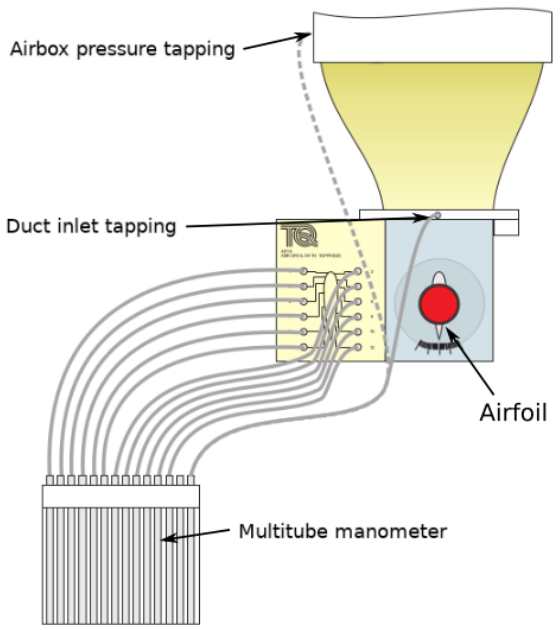
\includegraphics[scale=0.3]{fig/AF18.png}
    \caption{Pressure tappings for AF18 Experiment}
    \label{demo}
\end{figure}
